\documentclass[10pt,x11names,table]{beamer}

\usetheme[progressbar=frametitle]{metropolis}
\usepackage{appendixnumberbeamer}
\usepackage{xcolor}

\usepackage{polyglossia}
\setmainlanguage{spanish}

\usepackage{listings}

\usepackage{booktabs}
\usepackage[scale=2]{ccicons}

\usepackage{pgfplots}
\usepgfplotslibrary{dateplot}

%ANIMACIONES
\usepackage{animate}
\usepackage{graphicx}
\usepackage[caption=false]{subfig}

\usepackage{xspace}

\newcommand*{\eg}{e.g.\@\xspace}
\newcommand*{\ie}{i.e.\@\xspace}

\let\oldquote\quote
\let\endoldquote\endquote
\renewenvironment{quote}[2][]
  {\if\relax\detokenize{#1}\relax
     \def\quoteauthor{#2}%
   \else
     \def\quoteauthor{#2~---~#1}%
   \fi
   \oldquote}
  {\par\nobreak\smallskip\hfill(\quoteauthor)%
   \endoldquote\addvspace{\bigskipamount}}
   
\usepackage{wrapfig}

\usepackage{subfig}
\usepackage{hyperref}
\usepackage{multicol}

\setbeamertemplate{bibliography item}[text]

\usepackage[font=small,skip=0pt, labelformat=empty]{caption}

\usepackage{dirtytalk}
\usepackage[acronym]{glossaries}
\makeglossaries

\newacronym{acgan}{ACGAN}{Auxiliary Classifier GAN}
\newacronym{ae}{AE}{Autoencoder}
\newacronym{ai}{AI}{Artificial Intelligence}
\newacronym{api}{API}{Application Programming Interface}
\newacronym{bert}{BERT}{Bidirectional Encoder Representations from Transformers}
\newacronym{brief}{BRIEF}{Binary Robust Independent Elementary Features}
\newacronym{brnn}{BRNN}{Bidirectional RNN}
\newacronym{bptt}{BPTT}{Backpropagation Through Time}
\newacronym{cbow}{CBOW}{Continous bag-of-words}
\newacronym{cnn}{CNN}{Convolutional Neural Network}
\newacronym{crnn}{CRNN}{Convolutional Recurrent Neural Network}
\newacronym{ddpm}{DDPM}{Denoising Diffusion Probabilistic Model}
\newacronym{ddim}{DDIM}{Denoising Diffusion Implicit Model}
\newacronym{diffit}{DiffiT}{Diffusion Vision Transformer}
\newacronym{dl}{DL}{Deep Learning}
\newacronym{dnn}{DNN}{Deep Neural Network}
\newacronym{dos}{DoS}{Denial of Service}
\newacronym{drnn}{DRNN}{Deep Recurrent Neural Network}
\newacronym{ecg}{ECG}{Electrocardiogram}
\newacronym{elmo}{ELMo}{Embedding from Language Model}
\newacronym{fast}{FAST}{Features from Accelerated Segment Test}
\newacronym{fid}{FID}{Fréchet Inception Distance}
\newacronym{foss}{FOSS}{Free and open-source software}
\newacronym{gan}{GAN}{Generative Adversarial Network}
\newacronym{glove}{GloVe}{Global Vectors for Word Representation}
\newacronym{gpu}{GPU}{Graphics Processing Unit}
\newacronym{gru}{GRU}{Gated Recurrent Unit}
\newacronym{ilsvrc}{ILSVRC}{ImageNet Large Scale Visual Recognition Challenge}
\newacronym{is}{IS}{Inception Score}
\newacronym{kid}{KID}{Kernel Inception Distance}
\newacronym{ldm}{LDM}{Latent Diffusion Model}
\newacronym{lstm}{LSTM}{Long Short-Term Memory}
\newacronym{mape}{MAPE}{Mean Absolute Perentage Error}
\newacronym{ml}{ML}{Machine Learning}
\newacronym{mlp}{MLP}{Multilayer Perceptron}
\newacronym{mmd}{MMD}{Maximum Mean Discrepancy}
\newacronym{mse}{MSE}{Mean Squared Error}
\newacronym{ner}{NER}{Named Entity Recognition}
\newacronym{nlg}{NLG}{Natural Language Generation}
\newacronym{nlp}{NLP}{Natural Language Processing}
\newacronym{nlu}{NLU}{Natural Language Understanding}
\newacronym{nn}{NN}{Neural Network}
\newacronym{ocr}{OCR}{Optical Character Recognition}
\newacronym{onnx}{ONNX}{Open Neural Network Exchange}
\newacronym{pmml}{PMML}{Predictive Model Markup Language}
\newacronym{relu}{ReLU}{Rectified Linear Unit}
\newacronym{rest}{REST}{Representational State Transfer}
\newacronym{rnn}{RNN}{Recurrent Neural Network}
\newacronym{sae}{SAE}{Stacked Autoencoder}
\newacronym{sift}{SIFT}{Scale-Invariant Feature Transform}
\newacronym{slam}{SLAM}{Simultaneous Localization and Mapping}
\newacronym{sru}{SRU}{Single Recurrent Unit}
\newacronym{surf}{SURF}{Speeded-Up Robust Features}
\newacronym{svm}{SVM}{Support Vector Machine}
\newacronym{vae}{VAE}{Variational Autoencoder}
\newacronym{vgg}{VGG}{Visual Geometry Group}
\newacronym{vit}{ViT}{Vision Transformer}
\newacronym{wsgi}{WSGI}{Web Server Gateway Interface}
\newacronym{xai}{XAI}{eXplainable Artificial Intelligence}
\newacronym{yolo}{YOLO}{You Only Look Once}
\newacronym{zsl}{ZSL}{Zero-shot Learning}
\subtitle{Métodos Generativos, curso 2024-2025}

\date{\today}
\author{Guillermo Iglesias, guillermo.iglesias@upm.es \newline
Jorge Dueñas Lerín, jorge.duenas.lerin@upm.es  \newline
Félix Fuentes Hurtado, felix.fuentes@upm.es}

\institute{Escuela Técnica Superior de Ingeniería de Sistemas Informáticos | UPM \newline
\hbox{} \newline \ccbysa \hspace{0.1pt} \ccNonCommercial}

%%%%%%%%%%%%%%%%%%%%%%%%%%%%%%%%%%%%%       
\title{Detección de objetos}

\begin{document}
\maketitle

\begin{frame}{Introducción}
Hasta ahora, la única \alert{aplicación} que se ha visto de las \alert{\glspl{cnn}} son los clasificadores. Sin embargo existe una variedad enorme de posibilidades a la hora de procesar imágenes.

Dicho esto, las redes que ya han sido estudiadas comparten ciertas características a la hora de \alert{procesar imágenes}:

\begin{itemize}
    \item Extracción de características.
    \item Modelos jerárquicos.
    \item Composición de redes profundas.
\end{itemize}

Todo esto puede ser \alert{trasladado} a otras aplicaciones de la \alert{visión por computador}.
\end{frame}

\begin{frame}{Introducción}
Durante esta sesión se estudiarán las siguiente aplicaciones de la visión por computador:
\begin{itemize}
    \item \alert{Segmentación semántica} (semantic segmentation).
    \item Segmentación de instancias (instance segmentation).
    \item Detección y localización de objetos (object localization and detection).
\end{itemize}

\begin{figure}
    \centering
    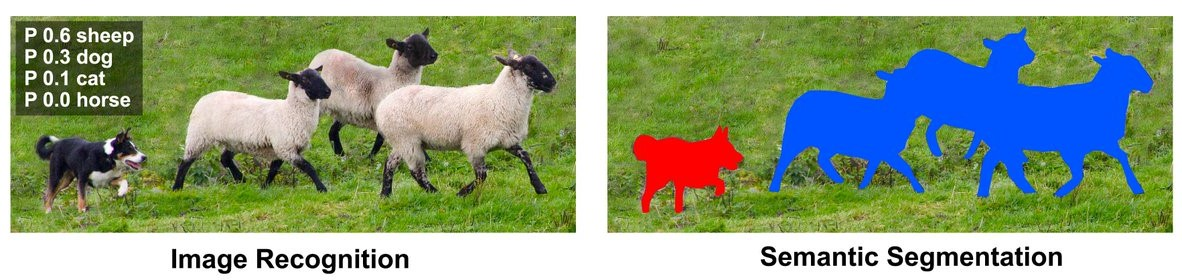
\includegraphics[width=\textwidth]{Slides/figures/Tema 4/SemanticSeg.jpg}
    \caption{\cite{SemanticSeg}}
\end{figure}
\end{frame}

\begin{frame}{Introducción}
Durante esta sesión se estudiarán las siguiente aplicaciones de la visión por computador:
\begin{itemize}
    \item Segmentación semántica (semantic segmentation).
    \item \alert{Segmentación de instancias} (instance segmentation).
    \item Detección y localización de objetos (object localization and detection).
\end{itemize}

\begin{figure}
    \centering
    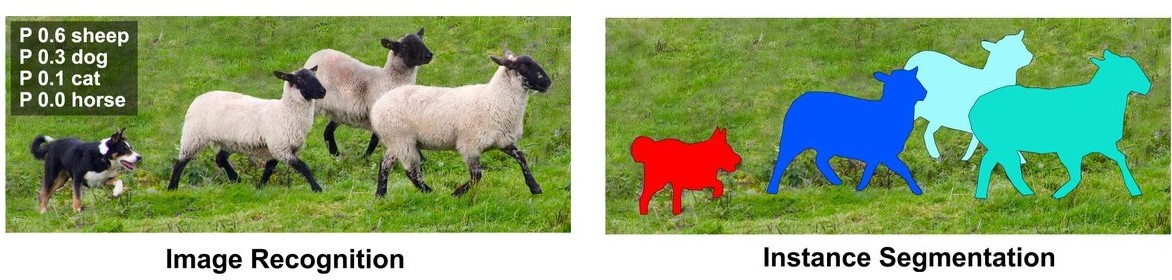
\includegraphics[width=\textwidth]{Slides/figures/Tema 4/InstanceSeg.jpg}
    \caption{\cite{InstanceSeg}}
\end{figure}
\end{frame}

\begin{frame}{Introducción}
Durante esta sesión se estudiarán las siguiente aplicaciones de la visión por computador:
\begin{itemize}
    \item Segmentación semántica (semantic segmentation).
    \item Segmentación de instancias (instance segmentation).
    \item \alert{Detección y localización de objetos} (object localization and detection).
\end{itemize}

\begin{figure}
    \centering
    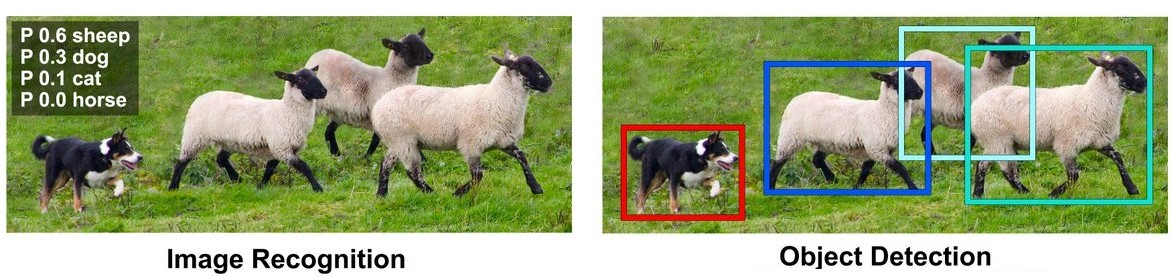
\includegraphics[width=\textwidth]{Slides/figures/Tema 4/ObjectDet.jpg}
    \caption{\cite{ObjectDet}}
\end{figure}
\end{frame}

\section{Segmentación semántica}

\begin{frame}{Definición del problema}
La \alert{segmentación semántica} consiste en realizar una \alert{clasificación} de cada uno de los \alert{píxeles} que conforman una imágen.

De esta manera se le asigna a cada píxel una \alert{etiqueta}, correspondiente al tipo de objeto que está \alert{representando}.

Cada una de las \alert{salidas de la red} representa una \alert{clasificación multi-clase} de los distintos posibles objetos presentes en la imagen. De esta manera cada uno de los \alert{píxeles de salida} se activa con una función \alert{softmax}.
\end{frame}

\begin{frame}{Ventana deslizante}
Uno de los modelos más \alert{sencillos} a la hora de realizar segmentación es utilizar un \alert{clasificador} que reciba cada una de las posibles ventanas de la imagen. Por cada ventana este realizará una \alert{clasificación} del los píxeles contenidos en ella.

\begin{figure}
    \centering
    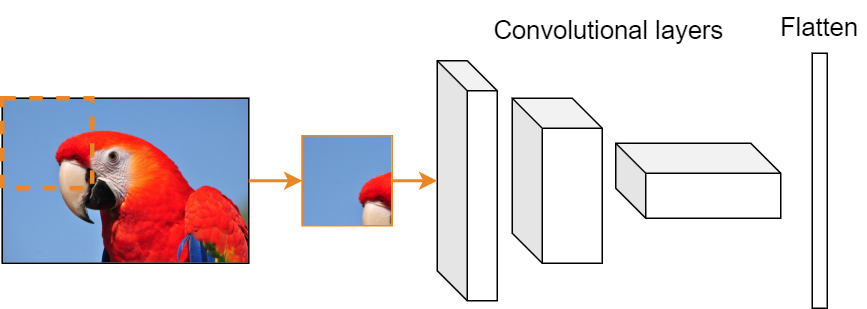
\includegraphics[width=\textwidth]{Slides/figures/Tema 4/SlidingWindow.png}
\end{figure}
\end{frame}

\begin{frame}{Ventana deslizante}
Uno de los modelos más \alert{sencillos} a la hora de realizar segmentación es utilizar un \alert{clasificador} que reciba cada una de las posibles ventanas de la imagen. Por cada ventana este realizará una \alert{clasificación} del los píxeles contenidos en ella.

\begin{figure}
    \centering
    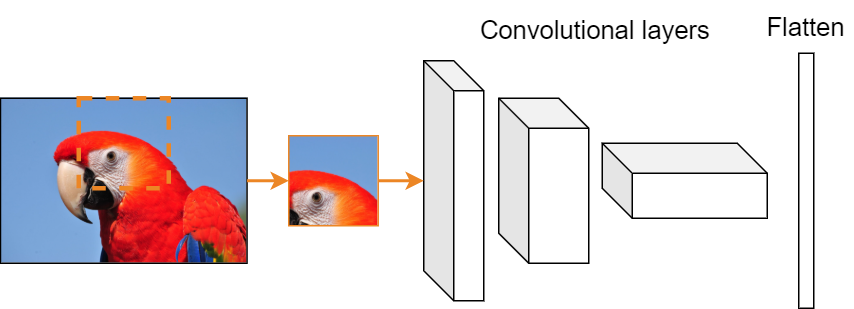
\includegraphics[width=\textwidth]{Slides/figures/Tema 4/SlidingWindow_1.png}
\end{figure}
\end{frame}

\begin{frame}{Ventana deslizante}
Sin embargo esta aproximación tiene multitud de inconvenientes:
\begin{itemize}
    \item \alert{Ineficiencia computacional}.
    \item \alert{Sólo es capaz de analizar una porción pequeña de la imagen}.
    \item \alert{Pérdida de información}.
\end{itemize}
\end{frame}

\begin{frame}{Red completamente convolucional}
Una \alert{\gls{cnn} estándar} está compuesta por una serie de capas convolucionales, seguidas de capas de Pooling y finalmente un \alert{perceptrón multicapa} para realizar predicciones.

\begin{figure}
    \centering
    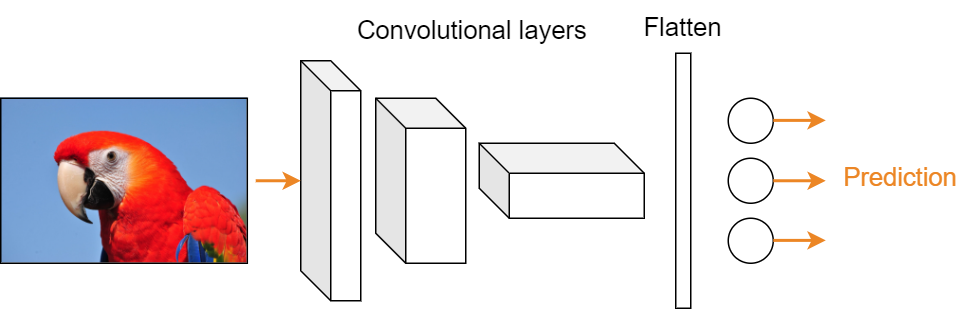
\includegraphics[width=\textwidth]{Slides/figures/Tema 4/StandardCNN.png}
\end{figure}
\end{frame}

\begin{frame}{Red completamente convolucional}
Pero a la hora de realizar \alert{segmentación semántica} no es necesaria la sección del \alert{perceptrón}, ya que no se va a predecir la etiqueta de la imagen.

Una red \alert{completamente convolucional} (fully convolutional \gls{cnn})\cite{long2015fully} elimina esta parte de la red, usando únicamente capas convolucionales.

\begin{figure}
    \centering
    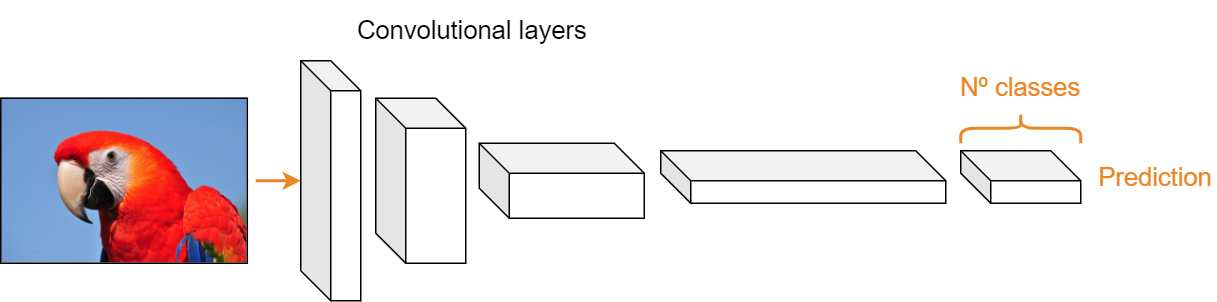
\includegraphics[width=\textwidth]{Slides/figures/Tema 4/FullyCNN.png}
\end{figure}

\textit{* la última capa se encarga de realizar la predicción para cada sección de la imagen, a través de una activación softmax.}
\end{frame}

\begin{frame}{Red completamente convolucional}
Las ventajas de esta arquitectura son:
\begin{itemize}
    \item Puede tratar \alert{imágenes de cualquier tamaño}.
    \item \alert{Eficiencia computacional} y de \alert{parámetros}.
    \item Reutilización de \alert{información}.
    \item Campo receptivo \alert{grande}.
\end{itemize}

\begin{figure}
    \centering
    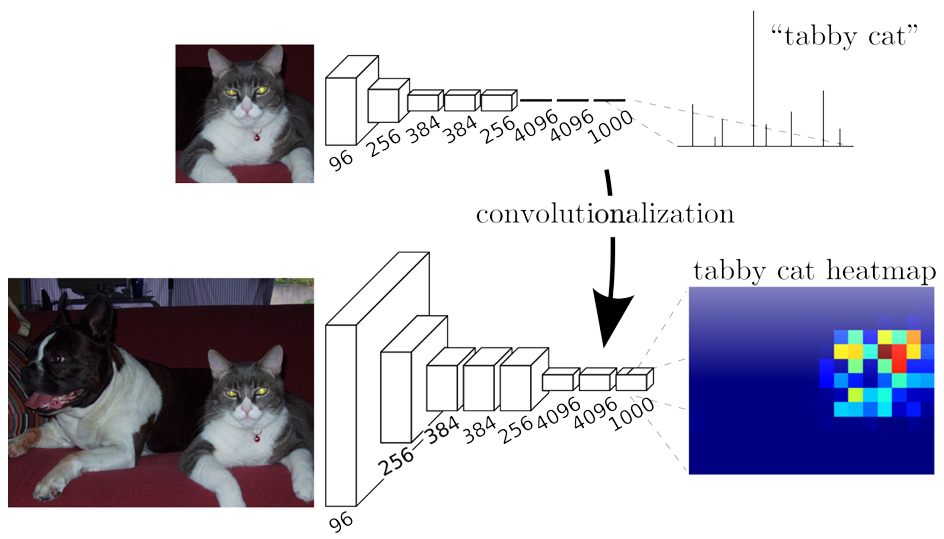
\includegraphics[width=0.7\textwidth]{Slides/figures/Tema 4/FullyCNNPaper.png}
    \caption{\cite{long2015fully}}
\end{figure}
\end{frame}

\begin{frame}{Autoencoder}
Una \alert{mejor solución} para realizar segmentación semántica es el uso de \alert{autoencoders}, propuesta con la red \alert{SegNet}\cite{badrinarayanan2015segnet}.

La estructura de \alert{encoder-decoder} permite extraer la información más relevante de la imagen y \alert{reconstruir} la misma \alert{identificando los elementos} que aparecen en ella.

\begin{figure}
    \centering
    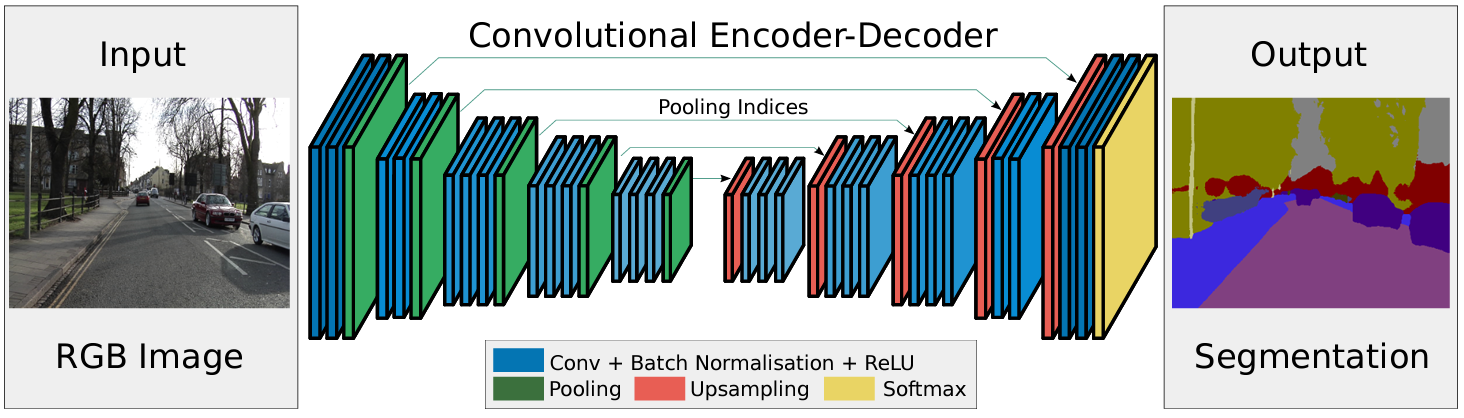
\includegraphics[width=\textwidth]{Slides/figures/Tema 4/SegNet.png}
    \caption{\cite{badrinarayanan2015segnet}}
\end{figure}
\end{frame}

\begin{frame}{UpSampling2D}
Para realizar el \alert{cambio de dimensionalidad} ascendente existen distintas alternativas.

\begin{figure}
    \centering
    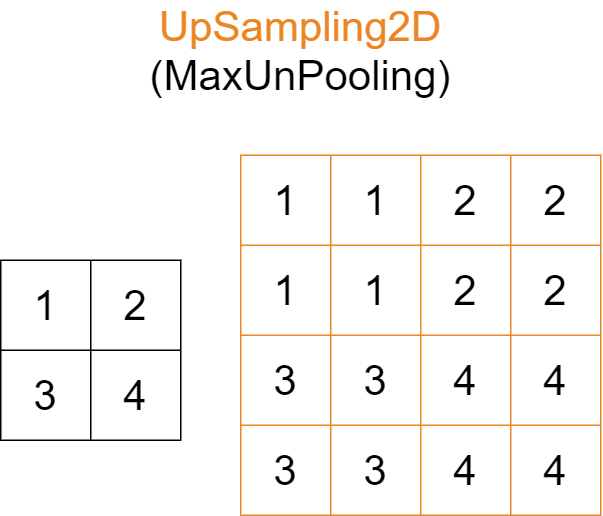
\includegraphics[width=0.5\textwidth]{Slides/figures/Tema 4/UpSampling2D.png}
\end{figure}
\end{frame}

\begin{frame}{Bed of nails unpooling}
Para realizar el \alert{cambio de dimensionalidad} ascendente existen distintas alternativas.

\begin{figure}
    \centering
    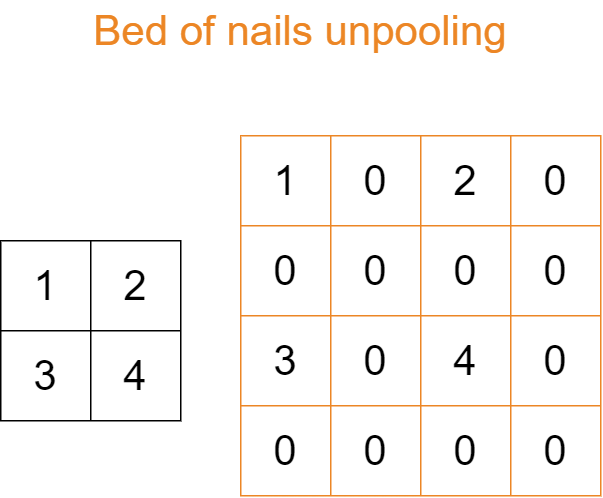
\includegraphics[width=0.5\textwidth]{Slides/figures/Tema 4/BedOfNails.png}
\end{figure}
\end{frame}

\begin{frame}{Bed of nails unpooling}
Esta arquitectura también propone un nuevo mecanismo para realizar \alert{UpSampling} de la información.

\begin{figure}
    \centering
    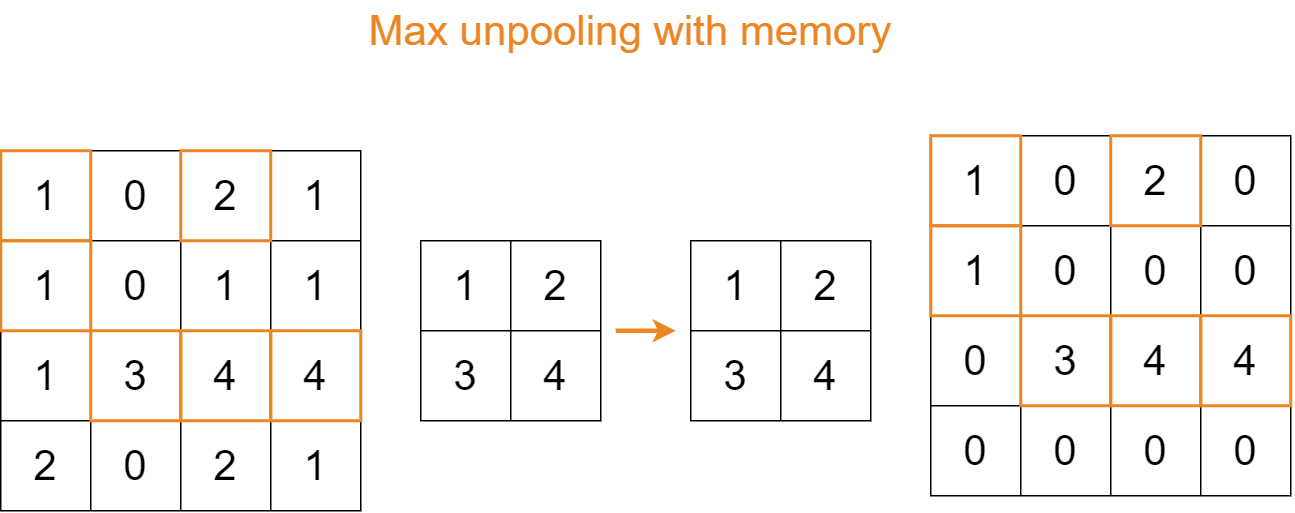
\includegraphics[width=\textwidth]{Slides/figures/Tema 4/MaxWithMemory.png}
\end{figure}
\end{frame}

\begin{frame}{Autoencoder}
Algunas de las características de esta arquitectura son:
\begin{itemize}
    \item Uso de \alert{\gls{vgg}} como arquitectura de referencia para el \alert{encoder}.
    \item MaxPooling \alert{con memoria}.
    \item \alert{Batch normalization} y \alert{ReLU} como activación.
\end{itemize}

\begin{figure}
    \centering
    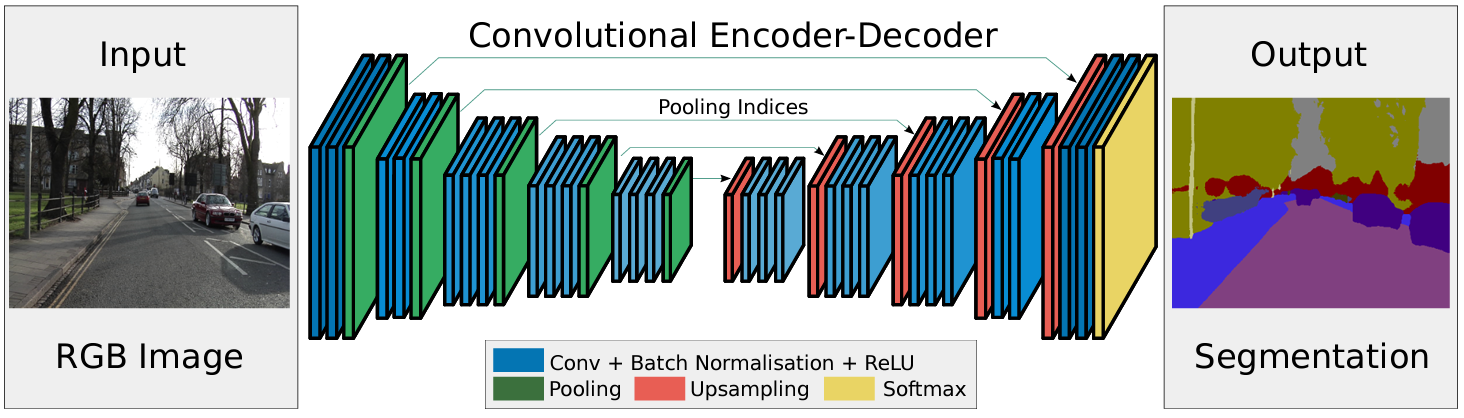
\includegraphics[width=\textwidth]{Slides/figures/Tema 4/SegNet.png}
    \caption{\cite{badrinarayanan2015segnet}}
\end{figure}
\end{frame}

\begin{frame}{U-Net}
La arquitectura \alert{U-Net}\cite{ronneberger2015u} tiene como objetivo conseguir \alert{imágenes de salida} con una mayor definición. Para ello se definen ciertas \alert{skip connections} con el objetivo de no \alert{perder información} sobre la composición de la imagen.

\begin{figure}
    \centering
    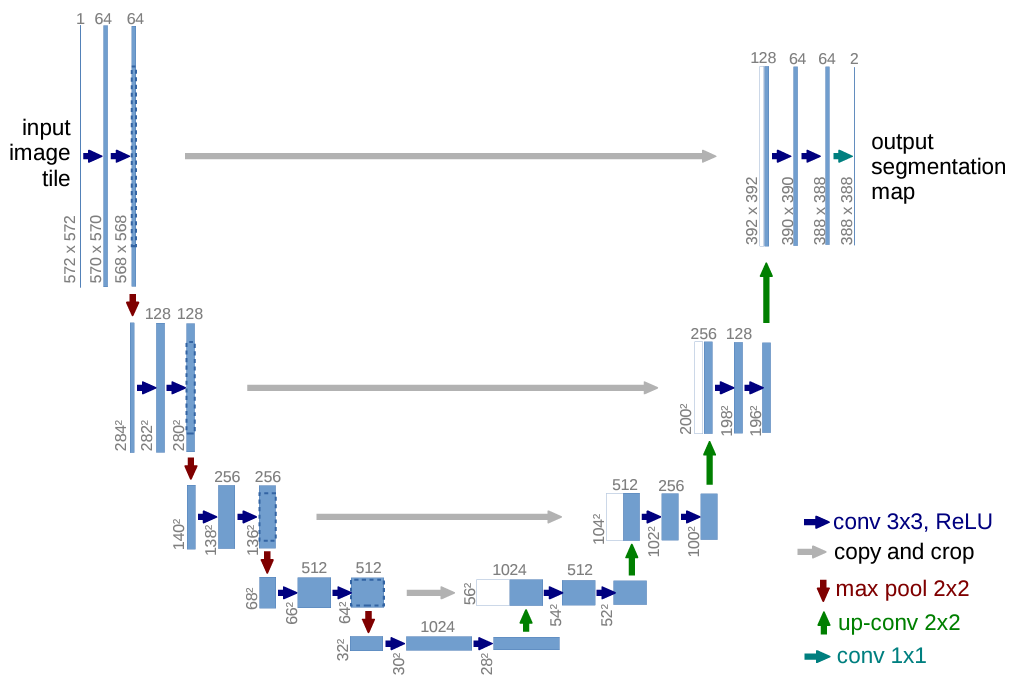
\includegraphics[width=0.7\textwidth]{Slides/figures/Tema 4/U-Net.png}
    \caption{\cite{ronneberger2015u}}
\end{figure}
\end{frame}

\section{Localización y detección de objetos}

\begin{frame}{Clasificación y localización}
La \alert{solución más simple} para realizar detección de objetos consiste en dividir la salida en \alert{dos tareas distintas}:
\begin{itemize}
    \item Clasificación de objetos
    \item Localización de objetos
\end{itemize}

\begin{figure}
    \centering
    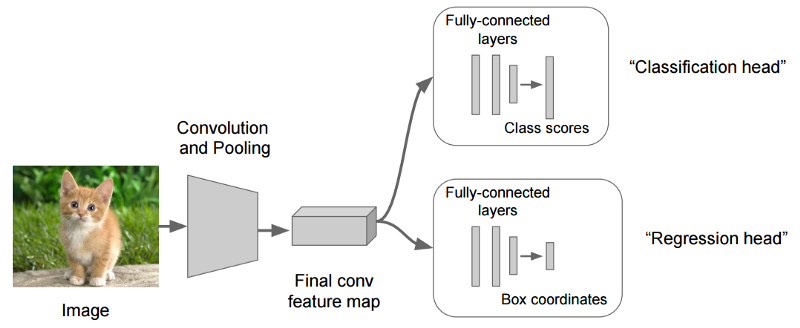
\includegraphics[width=\textwidth]{Slides/figures/Tema 4/ClasificationLocalization.png}
    \caption{\cite{ClaLocal}}
\end{figure}
\end{frame}

\begin{frame}{Detección de objetos}
Existen dos grandes ramas a la hora de tratar con la \alert{detección de objetos}:
\begin{itemize}
    \item \alert{Enfoques de una etapa}.
    \item \alert{Enfoques de dos etapas}.
\end{itemize}

\begin{figure}
    \centering
    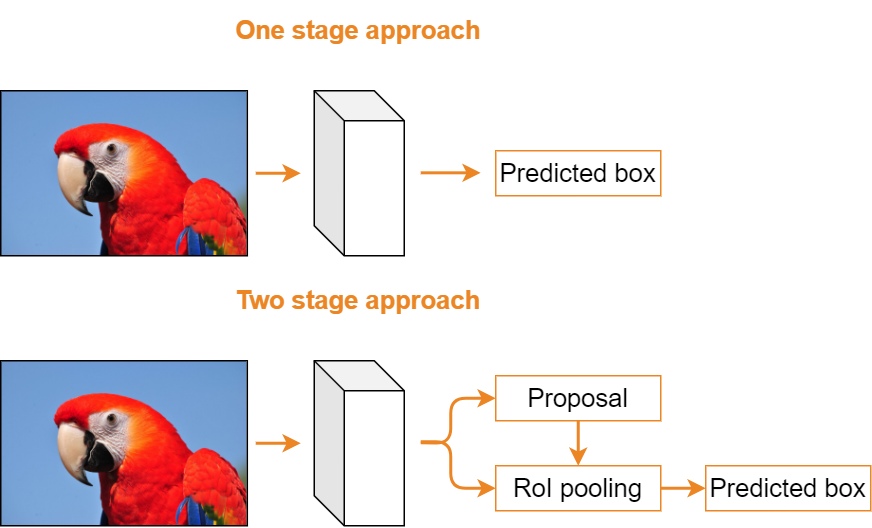
\includegraphics[width=0.8\textwidth]{Slides/figures/Tema 4/StageApproaches.png}
\end{figure}
\end{frame}

\begin{frame}{Faster R-CNN}
La arquitectura \alert{Faster R-CNN}\cite{ren2015faster} es una arquitectura en \alert{2 etapas}.

\begin{figure}
    \centering
    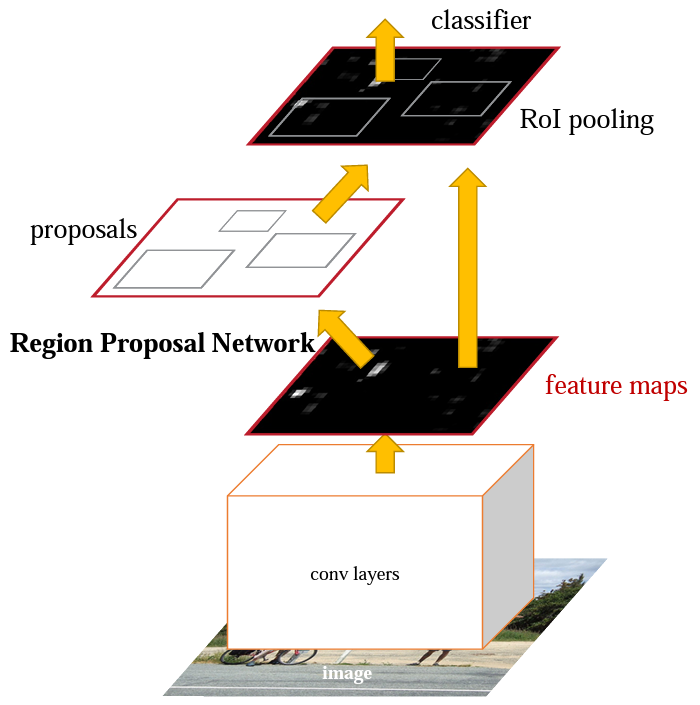
\includegraphics[width=0.6\textwidth]{Slides/figures/Tema 4/FasterRCNN.png}
    \caption{\cite{ren2015faster}}
\end{figure}
\end{frame}

\begin{frame}{Faster R-CNN}
La arquitectura se basa en \alert{2 redes neuronales}:
\begin{itemize}
    \item \alert{Region Proposal Network}: realiza predicciones a través de una \alert{ventana deslizante}.
    \item \alert{Feature Pyramid Network}: Se encarga de generar bounding boxes de mayor calidad.
\end{itemize}

\begin{figure}
    \centering
    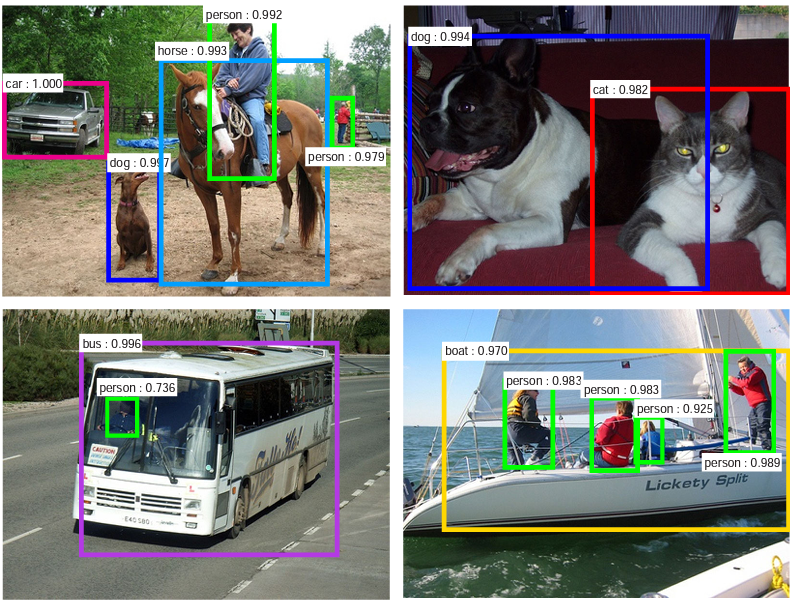
\includegraphics[width=0.6\textwidth]{Slides/figures/Tema 4/FasterRCNN_Results.png}
    \caption{\cite{ren2015faster}}
\end{figure}
\end{frame}

\begin{frame}{\gls{yolo}}
La arquitectura de \alert{\gls{yolo}} está compuesta por \alert{24 capas} con estilo de \alert{\gls{vgg}}.

\begin{figure}
    \centering
    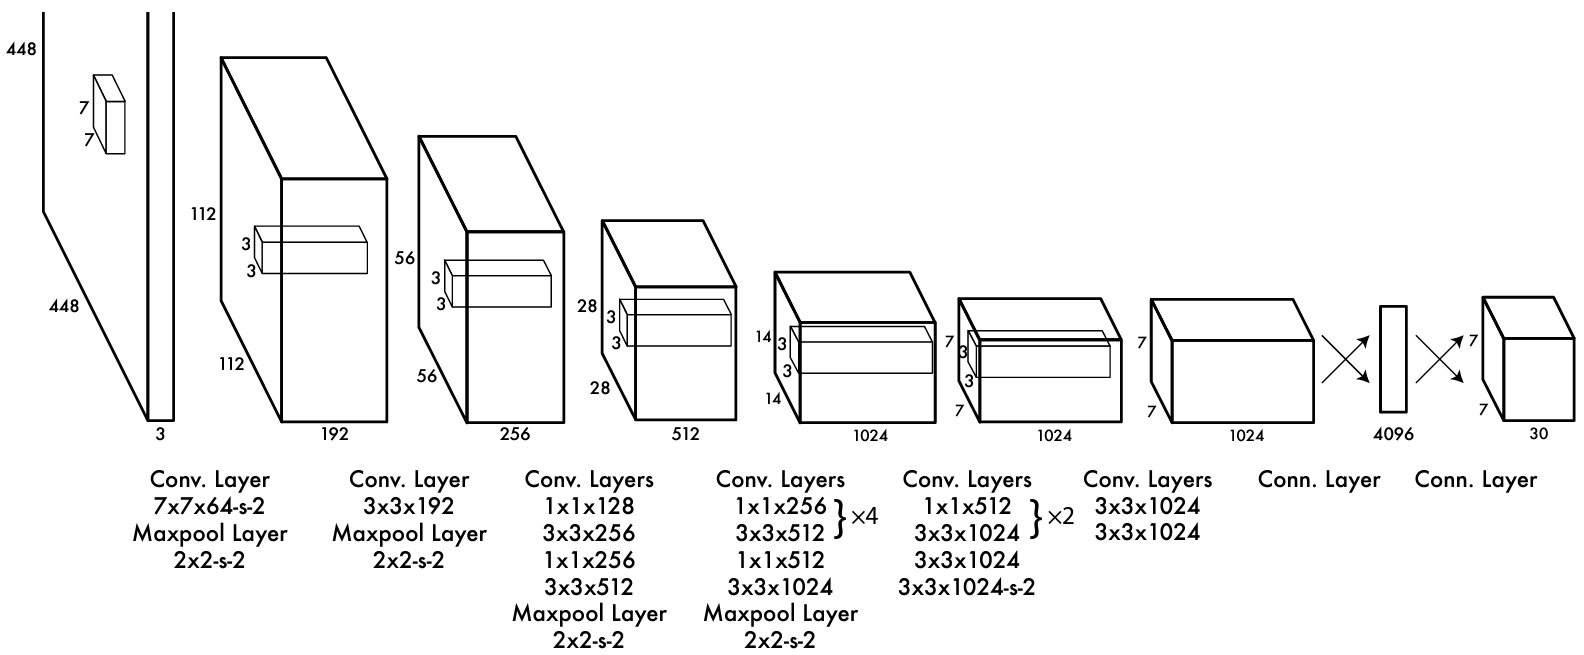
\includegraphics[width=\textwidth]{Slides/figures/Tema 4/YOLO_Architecture.png}
    \caption{\cite{redmon2016you}}
\end{figure}
\end{frame}

\begin{frame}{\gls{yolo}}
La \alert{última capa} de la red se encarga de \alert{predecir} dos \alert{bounding boxes} por cada \alert{ventana} de 7x7.

\begin{figure}
    \centering
    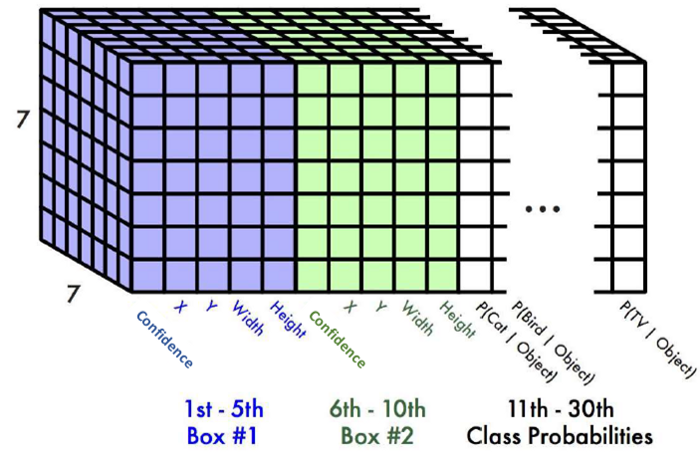
\includegraphics[width=0.8\textwidth]{Slides/figures/Tema 4/YOLO_End.png}
    \caption{\cite{YOLOFinal}}
\end{figure}
\end{frame}

\begin{frame}{\gls{yolo}}
Por cada división se calculan:
\begin{itemize}
    \item \alert{Dos bounding boxes}:
    \begin{itemize}
        \item 4 coordenadas de posición (x, y, w, h).
        \item 1 valor de confianza en la caja.
    \end{itemize}

    \item \alert{20 probabilidades de clase}
\end{itemize}

\begin{figure}
    \centering
    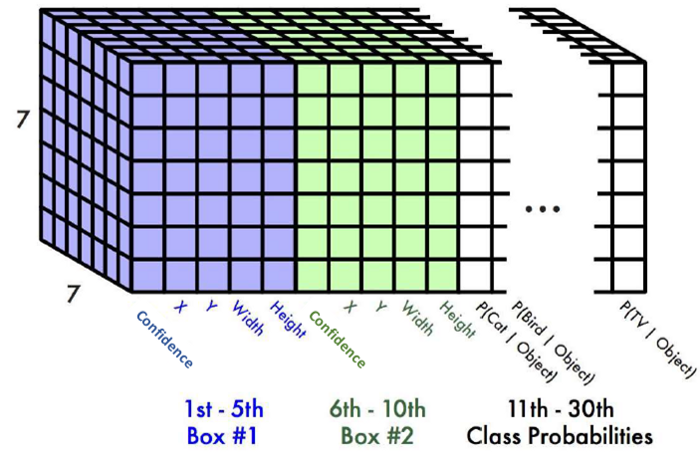
\includegraphics[width=0.7\textwidth]{Slides/figures/Tema 4/YOLO_End.png}
    \caption{\cite{YOLOFinal}}
\end{figure}
\end{frame}

\begin{frame}{\gls{yolo}}
Finalmente se realiza un \alert{depurado} de las \alert{bounding boxes} detectadas a través de \alert{non-maximum suppresion}.

\begin{figure}
    \centering
    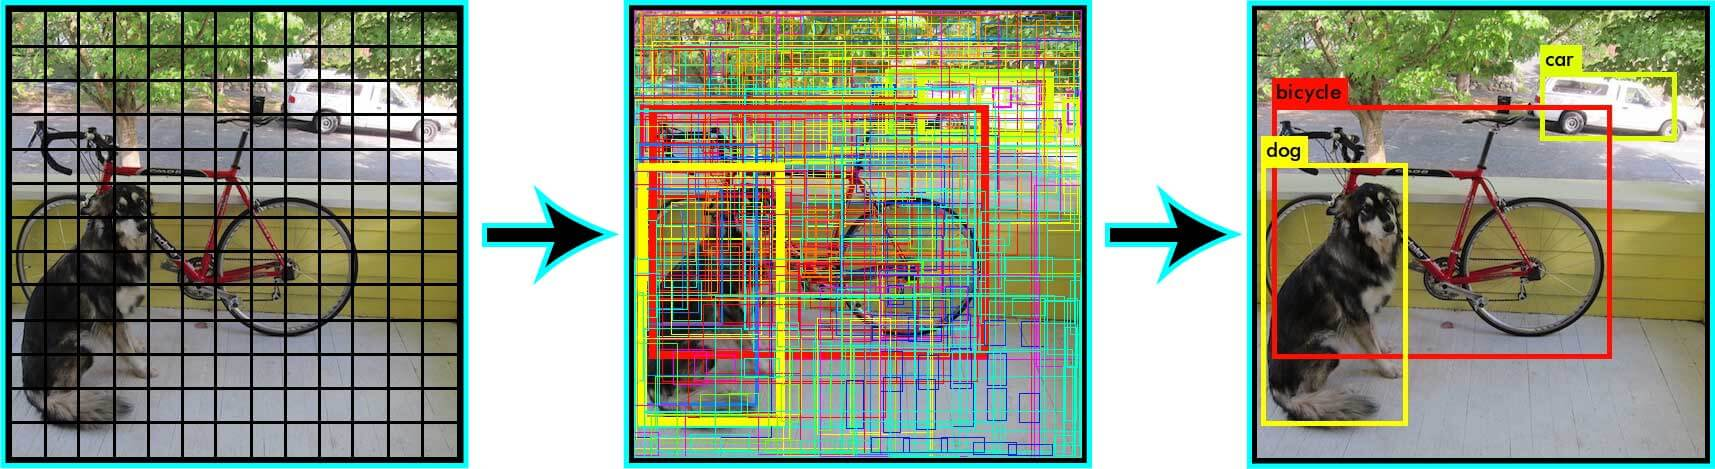
\includegraphics[width=\textwidth]{Slides/figures/Tema 4/YOLO_FinalResults.jpg}
    \caption{\cite{YOLOResults}}
\end{figure}
\end{frame}

\addcontentsline{toc}{section}{Referencias}

\begin{frame}[allowframebreaks]{Referencias}
    \bibliographystyle{unsrt}
    \bibliography{Slides/references.bib}
\end{frame}

\begin{frame}{Contribuciones de las diapositivas}
\begin{itemize}
    \item \textbf{Autor original de las diapositivas:} Guillermo Iglesias Hernández
    \item \textbf{Extensión de contenido:} Jorge Dueñas Lerín
\end{itemize}
\end{frame}

\end{document}